Riprenderei appunti di Russo e basta. Riportiamo cmq quello che dice lei.
Ci sono quattro principi base nella relatività.
\begin{itemize}
    \item Ogni legge fisica è invariante in ogni sistema di riferimento inerziale.
    \item Energia, impulso, momento angolare in ogni sistema fisica isolato si conservano.
    \item La velocità della luce è la stessa in ogni sistema di riferimento.
    \item Il tempo non è invariante (assoluto).
    \item I primi due sono legati alla meccanica classica, gli ultimi due alla relatività. Da ciò ne segue che le trasformazioni galileiane non valgono più, e al loro posto ci sono le trasformazioni di Lorentz. Nel limite $\beta\ll1$ le trasformazioni di Lorentz diventano quelle di Galileo.
\end{itemize}
\subsection{Trasformazioni di Lorentz}
\begin{itemize}
    \item Definiamo i quadrivettori come $A=(a_0,a_i)=(a_0,\vec a)$, con $a_0$ componente temporale e $a_i$ componente spaziale.
    \item Definiamo il prodotto scalare tra quadrivettori come $\tilde A\tilde B =a_0b_0-a_ib_i$. Questo prodotto è invariante sotto trasformazioni di Lorentz.
    \item Se consideriamo un sistema di riferimento $S$ e un altro $S'$, con $S'$ che si muove rispetto a $S$ con velocità $v$ lungo l'asse $x$, allora le trasformazioni di Lorentz sono date da:
    \begin{equation*}
        \mqty(a'_0 \\\xmat*{a'}{3}{1})= 
        \underbrace{\begin{pmatrix}
            \mqty{\gamma & -\beta\gamma & 0 & 0 \\ -\beta\gamma & \gamma &0&0 \\ 
            0 & 0 & 1 & 0 \\ 
            0 & 0 & 0 & 1 }
        \end{pmatrix}}_{=L(\beta)}
        \mqty(a_0 \\\xmat*{a}{3}{1})= 
        \mqty(\gamma a_0-\beta\gamma a_1\\-\beta\gamma a_0+\gamma a_1\\a_2\\a_3)\implies 
        \begin{cases}
            ct'=\gamma(ct-\beta x) \\
            x'=\gamma(x-\beta ct)
        \end{cases}
    \end{equation*}
    Una proprietà importante è $L(\beta)^{-1}=L(-\beta)$, da cui ne segue che per invertire le trasformazioni di Lorentz basta scambiare variabile con indice con quelle senza e $\beta\to-\beta$.
    \item Che si ha al limite non relativistico? Supponiamo $\beta\ll1\implies\gamma\approx1+\frac{\beta^2}{2}\approx1$. Ne segue per il tempo che
    \begin{equation*}
        ct'=\qty(1+\frac{\beta^2}2)(ct-\beta x) \approx ct-\beta x + \frac{\beta^2}2ct\approx ct\implies t'=t 
    \end{equation*}
    e per lo spazio che 
    \begin{equation*}
        x'=\qty(1+\frac{\beta^2}2)(x-\beta ct)\approx x-\beta ct\implies x'= x - vt
    \end{equation*}
    \item Se il moto non è solo lungo $x$, allora dobbiamo considerare $\vec\beta=\frac{\vec v} c$ e 
    \begin{equation*}
        \begin{cases}
            ct'=\gamma(ct-\beta x_\parallel) \\
            x'_\parallel=\gamma(x_\parallel-\beta ct)\\
            \vec x_\perp'=\vec x_\perp
        \end{cases}
    \end{equation*}
    \item Dimostriamo che il prodotto scalare è invariante. Sia $A=(a_0,\vec a)$ e $B=(b_0,\vec b)$. Calcoliamo $A'\cdot B'$.
    \begin{equation*}
        A'\cdot B'=a_0'b_0'-\vec a'\cdot\vec b'=\gamma^2(a_0-\beta a_1)(b_0-\beta b_1)-\gamma^2(a_1-\beta a_0)(b_1-\beta b_0)-a_2b_2-a_3b_3=\dots=A\cdot B
    \end{equation*}
\end{itemize}
Vediamo alcune conseguenze in high energy physics.
\begin{itemize}
    \item La contrazione delle lunghezze. Consideriamo un oggetto di lunghezza $L$ che si muove con velocità $v$. Supponiamo che il sistema solidale ad esso sia $S'$ e la lunghezza misurata sia $d'=x_2'-x_1'$ che avviene simultaneamente quindi $t_2=t_1$. Se trasformiamo otteniamo $d'=x_2'-x_1'=\gamma(x_2-\beta ct_2)-\gamma(x_1-bct_1)=\gamma(x_2-x_1)-\gamma\beta c(t_2-t_1)=\gamma(x_2-x_1)=d\implies d'=\gamma d$. Ne segue che la lunghezza misurata da un osservatore in moto è contratta di un fattore $\gamma$, e la lunghezza propria, misurata nel sistema solidale all'oggetto è la massima possibile.
    \item La dilatazione temporale. Consideriamo due eventi che avvengono nello stesso punto nello spazio, ma in tempi diversi. Se trasformiamo otteniamo $c\Delta t=c(t_2-t_1)=\gamma c(t_2'-t_1')+\beta \gamma (x_2'-x_1')=\gamma c\Delta t'$. Ne segue che il tempo misurato da un osservatore in moto è dilatato di un fattore $\gamma$, e il tempo proprio, misurato nel sistema solidale all'oggetto è il minimo possibile. Da ciò si hanno varie conseguenze.
\end{itemize}
\subsection{Esperimento CPP, muoni, pioni e Yukawa}
\begin{itemize}
    \item Nel 1912 Hess scoprì i raggi cosmici. Nel 1932 Anderson scoprì i positroni, predetti da Dirac nel 1928 (già discussa).
    \item Nel 1935 Yukawa introdusse la teoria delle interazioni forti, predicendo una massa mediatrice di $\sim 100$ MeV. Il mesone di Yukawa doveva decadere in elettrone e netruino con tempo di decadimento di $\sim1\mu$s. Nel 1937 si scoprì il mesotrone (Anderson e Neddermeyer), con una massa di $110$ MeV, associata alla particella di Yukawa. Nel 1940 si studiò assorbimento e decadimento delle proprietà di assorbimento del mesone di Yukawa.
    \item Il decadimento del mestrone (che in realtà è un $\mu$) fu studiato diverse volte. Nel 1940 si osservò il suo decadimento in positroni; nel 1941 ci fu una misura da Rasetti che ottenne $\tau=(1.5\pm0.3)\mu$s. Nel 1941 Piccioni e Conversi decisero di lavorare assieme e migliorare la precisione nella misura del tempo di decadimento (del mesone di Yukawa).
    \item Nel 1939 Montgomery fece un esperimento (\autoref{fig:montgomery}) per misurare il decadimento del $\mu$
    \begin{figure}[h]
        \centering
        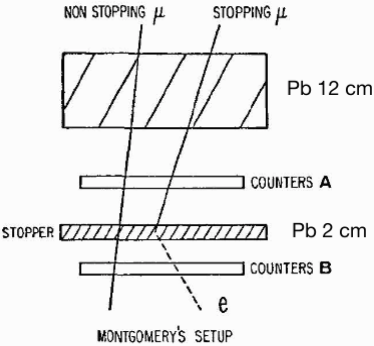
\includegraphics[width=0.4\textwidth]{immagini/fig_montgomery.png}
        \caption{Esperimento di Montgomery. Volevano estrarre il tempo di decadimento dalle intensità delle coincidenze ritardate con e senza stopper. Purtroppo non riuscirono a misurare il tempo di decadimento del $\mu$ a causa del troppo rumore in B.}
        \label{fig:montgomery}
    \end{figure}
    \item Un altro tentativo fu fatto da Rasetti nel 1940, con un apparato più complicato (\autoref{fig:rasetti}).
    \begin{figure}[h]
        \centering
        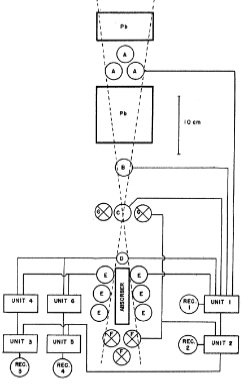
\includegraphics[width=0.4\textwidth]{immagini/fig_rasetti.png}
        \caption{Disposizione dei contatori, illustrando le connessioni con gli amplificatori.}
        \label{fig:rasetti}
      \end{figure}
    Nella procedura sperimentale si definisce un fascio di mestroni con la coincidenza ABCD. L'anticontatore G discrimina dagli sciami elettromagnetici. L'anticontatore F seleziona i mestroni che si sono fermati nell'assorbitore. Il contatore E rivela particelle emesse nell'assorbitore. Non si usarono coincidenze ritardate ma "immediate" con tempi di risoluzione diversi. Guardando le combinazioni dei tempi con cui il segnale arriva, hanno fatto un fit particolare ed estratto il tempo di decadimento. Ottennero $\tau=(1.5\pm0.3)\mu$s.
    \item Successivamente l'esperimento fu riproposto da Conversi, Pancini e Piccioni con l'idea di effettuare una misura migliore (vedi \autoref{fig:cpp})
    \begin{figure}[h]
        \centering
        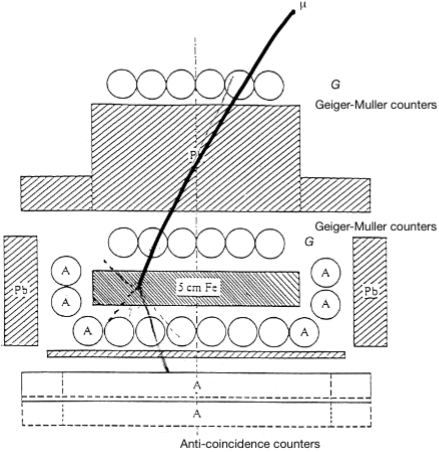
\includegraphics[width=0.4\textwidth]{immagini/fig_cpp.png}
        \caption{}
        \label{fig:cpp}
      \end{figure}
    Un mesotrone si ferma nell'assorbitore (Fe) e poi decade. Si usano coincidenze ritardate tra i contatori sopra e sotto e le anticoincidenze (A). Gli elettroni si fermano nell'assorbitore di Pb. Le anticoincidenze servono a scartare l'evento. Misurarono $\tau=(2.33\pm0.15)\mu$s, meglio di Rasetti. 
\end{itemize}
    Torniamo ai quadrivettori. 
    \begin{itemize}
    \item La matrice della metrica la conosciamo è $g^{\mu\nu}=\text{diag}(1,-1,-1,-1)$. Un quadrivettore importante è quello di impulso $P^\mu=(E,\vec p)$. Questo quadrivettore non è invariante ma il suo quadrato sì. Facendolo, scopriamo che vale $P^\mu P_\mu=m^2$ usando la relazione di mass-shell.
    \item Alcune relazioni utili sono: $p=\gamma mv$, $E=\gamma m$, $T=mc^2(\gamma-1)$, $\beta=\frac p E$.
    \item Quando facciamo esperimento di fisica di particelle, ci mettiamo nel riferimento di laboratorio solidale all'osservatore e ai rivelatori. In questo riferimento tipicamente $v\_T=0$. Possiamo scrivere allora nel riferimento del laboratorio $P_1=(E_1,\vec {p}_1)$, $P_2 = (m\_T,0)$ (1 = proiettile, 2 = target). Allora $P\_{tot}=sP_1+P_2=(E_1+m\_T,\vec p_1)$. 
    \item Un altro sistema di riferimento utile è quello del centro di massa, in cui $\vec {p}\_{tot}=0$. Se consideriamo una particella incidente in un target, avremo $P_1^*=(E_1^*,\vec p)$ e $P_2^*=(E_2^*,-\vec p)$. Allora $P\_{tot}^*=(E_1^*+E_2^*,0)$. Poichè è un invariante, $P\_{tot}^2$ sarà uguale nel riferimento del centro di massa e in quell del laboratorio. Ne segue che $P\_{tot}^{*,2}=E^2\_{CM}=P\_{tot}^{\text{lab},2}=(E_1+m\_T)^2-p_1^2=E_1^2+m\_T^2+2E_1m\_T-p_1^2=m_1^2+2E_1m\_T+m\_T^2$. ('sta roba è inutile?)
    \item Se consideriamo un fascio di $n$ particelle allora dovremo considerare la sommatoria. $P_\mu P^\mu= (E_1+E_2+\dots+E_n)^2-(\vec p_1+\vec p_2+\dots+\vec p_n)^2$ in generale. Se consideriamo il sistema del centro di massa avremo $P^{\mu,*}=(E\_{CM},0)$. Quindi nel riferimento del centro di massa questo scalare è solo il quadrato dell'energia nel sistema del centro di massa.
    \item Riprendiamo la storia. Nel 1947 ci fu la scoperta del pione, usando le emulsioni nucleari. Decade in sequenza il pione in muone ed infine in elettrone. In tutti gli eventi il muone aveva energia di 4.1 MeV a cui corrisponde il range misurato di 600 $\mu$m, le strisce sono tutte di uguale lunghezza (sappiamo da Bethe-Bloch che il range e l'impulso sono legati). In base a densità di ionizzazione ($\dd{E}/\dd{x}$) distinguiamo il tipo di particella.
    \item Visto che il range è sempre lo stesso, l'impulso del muone sarà sempre lo stesso 29 MeV. Visto che l'impulso è sempre lo stesso, il decadimento deve essere a due corpi (e non tre altrimenti si avrebbe spettro continuo). 
    \item Supponendo che si abbia un decadimento a due corpi con la particella iniziale che si ferma, abbiamo $X\to\mu+\nu_\mu$ e il sistema del centro di massa coincide con il sistema solidale a $X$ (il $\pi$). Da ciò ne segue che impulso di neutrino e muone sono uguali ed opposti, quindi  
    \begin{equation*}
    m\_X^2=E\_{cm}^2=(E_\mu+E_\nu)^2\implies m\_X=\sqrt{m_\mu^2+p_\mu^2}+p_\nu=\dots=138.9 \text{ MeV}
    \end{equation*}
    \item Il decadimento $\pi^-\to\mu^-+\bar\nu_\mu$ è dovuto alla forza debole, lo si capisce dal fatto che da quando avevo quark e antiquark, nei prodotti non li avrò più cioè non conservano il flavour. Un altro modo per capirlo è dai tempi di decadimento. 
    \begin{enumerate}
        \item Debole $10^{-8}-10^{-10}$ s.
        \item Elettromagnetico (come $\pi^0\to \gamma+\gamma$) $10^{-17}-10^{-16}$ s.
        \item Forti $10^{-22}-10^{-23}$ s.
    \end{enumerate}
\end{itemize}
Parliamo di processi virtuali e reali. 
\begin{itemize}
    \item Supponiamo di avere $e^-\to\gamma+e^-$. Abbiamo inizialmente (nel riferimento solidale all'elettrone) $e^-(m_ec^2,\vec0)$, invece dopo l'interazione abbiamo $e^-(E_k,-\vec k)+\gamma(c\abs{\vec k},\vec k)$. Valutiamo $\Delta E= ck+\sqrt{(m_ec^2)^2+(ck)^2}-m_ec^2$ consderando i due casi limite:
    \begin{enumerate}
        \item $ck\ll m_ec^2\implies \Delta E \gtrapprox ck$
        \item $ck\gg m_ec^2\implies \Delta E \lessapprox 2ck$
    \end{enumerate}
    Ne segue che 
    \begin{equation*}
        kc\leq\Delta E\leq2kc
    \end{equation*}
    ma ciò che importa è che $\Delta E\neq0$. Questo è un processo virtuale che non può avvenire da isolato. È possibile per un tempo compatibile con il principio di indeterminazione $t<\frac\hbar{\Delta E}$, a cui corrisponde uno spazio percorso $l=ct=\frac{c\hbar}{\Delta E}\propto(\Delta E)^{-1}$.
    \item Consideriamo un generico processo di scambio $A+B\to A+B$ che avviene tramite $X$. Avremo inizialmente $A(m_Ac^2,\vec0)$, invece dopo $A(E_p,\vec p)+X(E_X,-\vec p)$ e uguale per B. Vediamo quanto vale $\Delta E= E_X+E_p-m_Ac^2$ e i due casi limite:
    \begin{enumerate}
        \item $p\to\infty\implies \Delta E=2pc$
        \item $p\to0\implies\Delta E \geq m_Xc^2$
    \end{enumerate}
    ne segue che vale sempre $\Delta E\geq m_Xc^2$. Abbiamo detto che si può violare la conservazione dell'energia per $t\sim\frac\hbar{\Delta E}\implies l=\frac{c\hbar}{\Delta E}\approx\frac\hbar{m_X}$, dove $l$ è la massima distanza raggiungibile dal mediatore $X$ prima di essere ri-assorbito, e corrisponde esattamente al \textit{range della interazione}. 
    \item Viceversa, se conosco il range della interazione posso trovare la massa del mediatore! La relazione dunque è $R=\frac\hbar{m_Xc}$. Cerchiamo la massa del mediatore della interazione forte, supponendo che abbia $R\approx 1.2$ fm. Abbiamo 
    \begin{equation*}
    m_X=\frac1R=140\text{ MeV}
    \end{equation*}
    che è il mesotrone di Yukawa, chiamato così perché aveva massa intermedia tra $p$ ed $e^-$ (uniche particelle note oltre a $n$).
    \item Dunque se la massa del mediatore è nulla, il range dell'interazione è infinito (interazione elettromagnetica con fotoni). Se invece usiamo la massa del $W$, troviamo il range dell'interazione debole 
    \begin{equation*}
    R\_{debole}=\frac{\hbar c}{m_Wc^2}=\frac1{m_W}=\frac{200\text{ MeV}\cdot\text{fm}}{80\cdot 10^3\text{ MeV}}=2.5\cdot10^{-3}\text{ fm}
    \end{equation*}
    ben tre ordini di grandezza inferiori rispetto a quello nucleare.
    \item In passato si aveva una visione errata del $\beta$-decay, ad esempio $n\to p+e^-+\bar\nu$. In realtà questo avviene con uno scambio di $W^-$, cioè il neutrone (in realtà è tra quark) emette un $W^-$ diventando un $p$, e contemporaneamente $W^-\to e^-+\bar\nu$. Tuttavia questo processo lo trascuriamo a basse energie (MeV) in quanto irrilevante. 
\end{itemize}
Torniamo alla parte storica e all'esperimento CPP.
\begin{itemize}
    \item Abbiamo detto che l'esperimento CPP è importante perché da una migliore misura di $\tau_\mu$, ma c'è un altro motivo per cui è importante.
    \item Nel 1940 Tomonaga e Araki proposero una teoria, che fu accettata da tutti, sull'interazione forte. Il mesone di Yukawa interagisce con il nucleo mediante interazione forte. Secondo i calcoli, la cattura nucleare dipende leggermente dallo Z del materiale. I mesotroni positivi sono respinti dal nucleo, mentre quelli negativi possono essere catturati, ne segue che i mesotroni positivi possono soltanto decadere.
    \item  Per testare questa teoria che prevedeva una asimmetria tra mesotroni positivi e negativi, si usò lo stesso apparato CPP. La differenza stava in assorbitori più sottili (0.6 cm di Fe invece di 5 cm) per migliorare la efficienza di rivelazione degli elettroni. Misurarono il rapporto di mesotroni che decadono dentro il ferro che era in accordo con il valore aspettato (da raggi cosmici si aspettavano un eccesso del 20\%).
    \item Poi ripetettero l'esperimento con un apparato migliore utilizzando le lenti magnetiche per separare mesotroni positivi e negativi. Con un assorbitore ad alto Z (ferro) ci fu conferma della teoria, con uno a basso Z (carbonio), per completezza e per rivelare i fotoni emessi da cattura nucleare dei mesotroni negativi, invece ci fu disaccordo. Quindi la differenza è il campo magnetico che distingue i mesotroni positivi e negativi e utilizzo di assorbitori con alto e basso Z.
    \item Attraverso assorbitori di 5 cm di Fe c'è accordo perché la frequenza di decadimento è maggiore per quelli positivi non catturati rispetto a quelli negativi, il cui risultato sperimentale è compatibile con zero (vengono catturati dai nuclei prima di decadere). Il problema nasce con assorbitori di grafite, perché si trova che il rate di decadimento delle particelle negative non solo è diverso da zero, ma molto simile a quelle positive. Allora i mesotroni non sono le particelle di Yukawa, quelle che interagiscono fortemente.
    \item Fermi e altri discussero, e conclusero che ci sono circa 12 ordini di grandezza di differenza tra il tempo di cattura per una particella di Yukawa negativa e i risultati dell'esperimento. Quindi il mesotrone fu ribattezzato, come lo conosciamo oggi, mesone $\mu$, ed oggi sappiamo che il pione è la particella di Yukawa.
    \item Quindi CPP è rivoluzionario perché scopre che il muone non è la particella di Yukawa, quindi è un altro leptone! Apre la strada alla seconda generazione di particelle, con cui si va oltre la materia ordinaria. Quindi è l'inizio della \textit{fisica delle particelle}.
\end{itemize}
Vediamo il potenziale di \textit{Yukawa}.
\begin{itemize}
    \item Consideriamo $A+B\to A+B$ con particella mediatrice $X$. Questa particella è un bosone, se in più la consideriamo relativistica allora obbedisce all'equazione di Klein-Gordon. Nel caso statico (stazionario) si riduce a
    \begin{equation*}
        \nabla^2\phi(\vec x)=\frac{m_X^2c^2}{\hbar^2}\phi(\vec x)
    \end{equation*}
    se la massa è nulla ritroviamo l'equazione di Laplace e quindi il mediatore è il fotone e la soluzione è il campo elettrostatico $V(r)=-\frac{e^2}{4\pi\varepsilon_0}\frac1r$. Se invece la massa non è nulla otteniamo $V(r)=-\frac{g^2}{4\pi}\frac{e^{-r/R}}{r}$ che è il \textit{potenziale di Yukawa} con il range $R=\frac{\hbar}{m_Xc}$. La forma del potenziale è simile a quello che si ottiene quando consideriamo effetti di schermaggio e vogliamo la carica effettiva subita dal sistema.
    \item Ci sono delle ipotesi su cui si basa il modello di Yukawa.
    \begin{enumerate}
        \item I nucleoni sono le sorgenti del campo nucleare e l'interazione tra essi avviene tramite scambio di bosoni che quantizzano il campo nucleare (detti mesoni).
        \item L'interazione è a corto range, con range legato alla massa della particella mediatrice.
        \item L'interazione nucleare è indipendente dalla carica elettrica.
        \item Il potenziale è a simmetria sferica e dipende anche dagli spin dei nucleoni (che abbiamo ignorato).
    \end{enumerate}
\end{itemize}
Il modello di Yukawa serve anche a spiegare lo scattering $p-n$.
\begin{itemize}
    \item La distribuzione angolare di scattering protone-neutrone ha un andamento a parabola con picchi in 0 e 180 gradi (e minimo in mezzo da qualche parte). Senza il modello di Yukawa non è spiegabile.
    \item Se lo scattering è elastico $\abs{\vec p_i}=\abs{\vec p_f}$. L'impulso trasferito varrà $\Delta p = \abs{\vec p_i-\vec p_f}=F\_{media}\Delta t$. Considerando il potenziale nucleare come una buca, avremo $F\_{media}=\frac{V_0}R$. La variazione di impulso è legata all'angolo soltanto visto che è elastico, quindi  (usando $\Delta t=R/v$)
    \begin{equation*}
        \Delta \vartheta\approx \frac{\Delta p} p=\frac{F\_m\Delta t}p=\frac{V_0}{vp}\implies \vartheta=\frac{V_0}{2E\_{cin}}
    \end{equation*}
    usando il valore tipico di $V_0=35$ MeV e $100$ MeV $\leq E\_{cin}\leq600$ MeV (usati sperimentalmente) otteniamo $\vartheta=10$ gradi, che è in accordo con i dati sperimentali. 
    \item Quindi con la cinematica spieghiamo il picco ad angoli bassi, ma non quello ad angoli alti. Per spiegarlo dobbiamo considerare il modello di Yukawa, si scambiano un pione quindi esiste uno stato intermedio (non è puntuale, pensando a diagramma di Feynman senza mediatore).
\end{itemize}
\subsection{Scoperta dell'antiprotone}
\begin{itemize}
    \item Gli antiprotoni sono più difficili da rivelare rispetto ai positroni perché avranno una massa pari a quella del protone e quindi sono più difficile da produrre. Ovviamente ce li aspettiamo con massa negativa.
    \item Quindi come possiamo crearli? Da raggi cosmici non è possibile vederli. Serve un acceleratore e non deve essere collider. A quanta energia deve arrivare? Consideriamo la reazione $p+p\to p+p+\bar p+p$ e troviamo la energia di soglia.
    \item Calcoliamo l'energia di soglia nel caso in cui abbiamo inizialmente un proiettile $i$ contro un target $T$ fermo e si hanno $N$ particelle finali.
    \begin{equation*}
    \text{Iniziale}:\,E^2=(E_i+m_T)^2-p_i^2=\dots=m_i^2+m_T^2+2m_TE_i
    \end{equation*}
    \begin{equation*}
    \text{Finale}:\,E^2=\qty(\sum_{k=1}^N E_k+m_k)^2\geq\qty(\sum_km_k)^2
    \end{equation*}
    perché visto che voglio l'energia di soglia basta la loro "massa". Ne segue che 
    \begin{equation*}
    m_i^2+m_T^2+2m_TE_i\geq\qty(\sum_km_k)^2
    \end{equation*}
    Sostituendo $E_i=T_i+m_i$ risulta
    \begin{equation*}
    T_i\geq\frac{\qty(\sum_km_k)^2-(m_T+m_i)^2 } {2m_T}
    \end{equation*}
    Questa relazione ci da l'idea di quanta energia devo dare alla particella incidente per produrre una certa reazione.
    \item Applichiamolo al nostro caso per produrre l'antiprotone.
    \begin{equation*}
    T_i\geq\frac{(4m_p)^2-(2m_p)^2}{2m_p}=5.6\text{ GeV}
    \end{equation*}
    Questo non va bene. Il problema è che abbiamo considerato il protone del target fermo, ma noi non abbiamo mai un protone libero.
    \item In questo particolare esperimento usarono rame come target, quindi il protone era confinato nel nucleo e si muove. Assumendo che in questa interazione interagiamo con quello della shell più esterna, questo avrà l'impulso di Fermi $p_F=0.24$ GeV. Questo complica il calcolo perché adesso c'è una certa distribuzione di energia in quanto questo impulso può essere orientato casualmente. Studiamo i casi limite in cui è parallelo e antiparallelo all'impulso della particella incidente.
    \item Nel riferimento del laboratorio abbiamo $P^\mu=(E_i+E_F,\vec p_i+\vec p_F)$, dunque
    \begin{equation*}
    \text{Iniziale: } P^\mu P_\mu=(E_i+E_F)^2-(\vec p_i+\vec p_F)^2=E_i^2+E_F^2+2E_iE_F-p_i^2-p_F^2-2\vec p_i\cdot\vec p_F
    \end{equation*}
    Applichiamo la relazione di mass-shell $E_{i,F}^2-p_{i,F}^2=m_{i,T}^2$ e consideriamo $\vec p_i\cdot\vec p_F=\pm p_ip_F$, dove il caso antiparallelo corrisponde al segno meno, che diventa positivo, e quindi corrisponde ad energia di soglia maggiore. Risulta
    \begin{equation*}
        2m_p^2+2E_pE_F\pm2p_pp_F\geq 16m_p^2
    \end{equation*}
    \item Facciamo un paio di considerazioni.
    \begin{enumerate}
        \item $E_F=m_p+\frac{p_F^2}{2m_p}$, cioè un approccio classico dovuto al fatto che l'energia di Fermi è bassa.
        \item $E_p\approx p_p$ che in realtà sarebbe $p=6$ GeV contro la massa del protone $m_p=1$ GeV ma approssimiamo lo stesso $p\gg m$. 
    \end{enumerate}
    Ne segue che 
    \begin{equation*}
        2m_p^2+2E_p\qty(m_p+\frac{p_F^2}{2m_p})\pm 2p_FE_p\geq 16m_p^2\implies\dots\implies
    \end{equation*}
    \begin{equation*}
        \implies E_p\geq\frac{7m_p}{1+\frac{p_F^2}{2m_p^2}\pm\frac{p_F}{m_p}}
    \end{equation*}
    \item A questo punto l'energia cinetica la ricaviamo da $T_p=E_p-m_p$ ottenendo 
    \begin{equation*}
    4.2\text{ GeV }\leq T_p\leq 7.5\text{ GeV }
    \end{equation*}
    Sono importanti sia il minimo che il massimo: il minimo perché altrimenti non riusciamo a vedere quello che desideriamo, il massimo perché costruire acceleratori che raggiungono alte energie è costoso (se possibile tecnologicamente). Segrè e l'altro fecero questo esperimento a 6.2 GeV, quindi non prendevano proprio tutti i casi in quanto non avevano la massima energia possibile, ma è un esperimento di scoperta quindi basta una rivelazione.
    \item Adesso che sappiamo che energia incidente serve, come riveliamo l'antiprotone? Tanto per cominciare dalla reazione $p+p$ possono succedere tante cose.
    \item Come prima cosa distinguiamo il segno delle cariche usando un campo magnetico. Adesso serve distinguere i $\pi^-$ da i $\bar p$.  I pioni veloci si possono tagliare tramite un rivelatore Cherenkov che dà un trigger solo se si ha una certa velocità e si scartano le particelle che lo attivano. Resta il problema dei pioni lenti. Per risolvere questo problema si misura il tempo di volo. \textbf{Appunti di albergo non capisco} e conoscendo tempo di volo e massa si può identificare l'antiprotone.
\end{itemize}
\subsection{Differenza target fisso e collider}
Bisogna fare attenzione a non confondere acceleratori circolari, in cui i ltarget è comunque fisso, con collider.
\begin{itemize}
    \item Nei collider di solito c'è particella contro antiparticella oppure particelle uguali. È Più efficiente produrre particelle in questo modo perché non spendo energia per spostare il centro di massa.
    \item Consideriamo target fisso. Abbiamo $P^\mu_1=(E_1,\vec p_1)$ e $P^\mu_2=(m_2,0)$. Calcoliamo la massa invariante (sommando i quadri-impulsi)
    \begin{equation*}
        s^2=P^\mu P_\mu=\qty(E_1+m_2)^2-p_1^2=\dots=m_1^2+m_2^2+2E_1m_2 \underset{m_{1,2}\ll E_1}{\implies} \sqrt s=\sqrt{2E_1m_2}
    \end{equation*}
    \item Consideriamo collider. In generale $P^\mu_1=(E_1,\vec p_1)$ e $P^\mu_2=(E_2,\vec p_2)$ da cui (di solito $E_1=E_2$)
    \begin{equation*}
        s^2=(E_1+E_2)^2-(\vec p_1+\vec p_2)^2=\dots=m_1^2+m_2^2+2(E_1E_2-\vec p_1\cdot \vec p_2)\underset{
            \begin{subarray}{c}
                m_{1,2}\ll E_1\\
                \abs{p_{1,2}}\approx E_{1,2}
             \end{subarray}}{\implies}
        s=2E^2(1-\cos\vartheta)
    \end{equation*}
    Da cui, visto che è un collider avremo $\vartheta=\pi\implies \sqrt s=2E$.
    \item Dunque, ricordando che $E\_{cm}=\sqrt s$, si avrà che l'energia a disposizone per creare nuove particelle sarà maggiore, a parità di energia del fascio, per il collider piuttosto che target fisso. 
    \item Possiamo fare un calcolo esplicito. Consideriamo un fascio di protoni a $E=100$ GeV. Nel caso di target fisso abbiamo
    \begin{equation*}
        \sqrt s=\sqrt{2E_1m_2}\approx 14\text{ GeV}
    \end{equation*}
    invece in un collider ho 
    \begin{equation*}
        \sqrt s=2E_1\approx 200\text{ GeV}
    \end{equation*}
    Quindi con un collider ho molta più energia a disposizione. Se volessi infatti avere a disposizione $200$ GeV a target fisso dovrei avere un fascio di energia
    \begin{equation*}
        200=\sqrt{2E}\implies E=2\cdot10^4\text{ GeV}
    \end{equation*}
    d'altra parte già dagli anni 70 si usano solo collider.
\end{itemize}
\subsection{Trasformazioni di Lorentz tra centro di massa e laboratorio}
\begin{itemize}
    \item Per un sistema di $n$ particelle abbiamo 
    \begin{equation*}
        P^\mu\_{lab}=\qty(\sum_kE_k,\sum_k\vec p_k)
    \end{equation*}
    \begin{equation*}
        P^\mu\_{cm}=\qty(\sum_kE_k^{\text{cm}},0)=(\sqrt s,0)
    \end{equation*}
    Se trasformiamo con Lorentz abbiamo 
    \begin{equation*}
        \mqty(\frac{\sqrt s} c \\ \zmat{3}{1})= 
        \begin{pmatrix}
            \mqty{\gamma\_{cm} & -\beta\_{cm}\gamma\_{cm} & 0 & 0 \\ -\beta\_{cm}\gamma\_{cm} & \gamma\_{cm} &0&0 \\ 
            0 & 0 & 1 & 0 \\ 
            0 & 0 & 0 & 1 }
        \end{pmatrix}
        \mqty(\sum_k\frac{E_k}c \\ \sum_k\vec p_k \\ \zmat{2}{1})\implies 
    \end{equation*}
    \begin{equation*}
        \implies 
        \begin{cases}
            \frac{\sqrt s}c=\gamma\_{cm}\sum_k\frac{E_k}c-\beta\_{cm}\gamma\_{cm}\sum_k\abs{\vec p_k}\\
            0=-\beta\_{cm}\gamma\_{cm}\sum_k\frac{E_k}c +\gamma\_{cm}\sum_k\abs{\vec p _k}
            \end{cases}
    \end{equation*}
    da cui $\beta\_{cm}=\frac{\abs{p\_{lab}^{\text{tot}}}}{E^{\text{tot}}\_{lab}}$ velocità del centro di massa, e $\gamma\_{cm}=\frac{E^{\text{tot}}\_{lab}}{\sqrt s}$ sempre del centro di massa.
    \item Si può anche fare al contrario da sistema del centro di massa a sistea del laboratorio. Stavolta abbiamo 
    \begin{equation*}
        P^\mu\_{lab}=\qty(E_1+m_2,\vec p_1)
    \end{equation*}
    \begin{equation*}
        P^\mu\_{cm}=\qty(\sum_kE_k^{\text{cm}},0)=(\sqrt s,0)
    \end{equation*}
    Se trasformiamo con Lorentz abbiamo 
    \begin{equation*}
        \mqty(E_1+m_2 \\ \zmat{2}{1}\\p_1)= 
        \begin{pmatrix}
            \mqty{\gamma\_{cm} & 0 & 0 & \beta\_{cm}\gamma\_{cm} \\ 0 & 1 &0&0 \\ 
            0 & 0 & 1 & 0 \\ 
            \beta\_{cm}\gamma\_{cm} & 0 & 0 & \gamma\_{cm} }
        \end{pmatrix}
        \mqty(\sqrt s \\ \zmat{3}{1})\implies 
    \end{equation*}
    \begin{equation*}
        \implies 
        \begin{cases}
            E_1+m_2=\gamma\_{cm}\sqrt s\\
            p_1=\beta\_{cm}\gamma\_{cm}\sqrt s
            \end{cases}
    \end{equation*}
    da cui $\beta\_{cm}=\frac{ p_1}{E_1+m_2}$ e $\gamma\_{cm}=\frac{E_1+m_2}{\sqrt s}$
\end{itemize}
\subsection{Impulso trasverso}
Normalmente nei collider si usano rivelatori a simmetria cilindrica o sferica. Vediamo le relazioni in termini di coordinate sferiche.
\begin{itemize}
    \item Assumiamo che il centro di massa si muova lungo $z$, e passiamo dal riferimento del centro di massa a quello del laboratorio. Indichiamo con $^*$ le quantità nel riferimento del centro di massa.
    \begin{equation*}
    P^\mu=\mqty(E\\p_x\\p_y\\p_z)=\mqty(E\\p\sin\vartheta\cos\varphi\\p\sin\vartheta\sin\varphi\\p\cos\vartheta)=
    \begin{pmatrix}
        \mqty{\gamma & 0 & 0 & \beta\gamma \\ 0 & 1 &0&0 \\ 
        0 & 0 & 1 & 0 \\ 
        \beta\gamma & 0 & 0 & \gamma }
    \end{pmatrix}
    \mqty(E^*\\p^*\sin\vartheta^*\cos\varphi^*\\p\sin\vartheta^*\sin\varphi^*\\p\cos\vartheta^*)\implies
    \end{equation*}
    
    \begin{equation*}
        \implies 
        \begin{cases}
            E=\gamma E^*+\beta\gamma p^*\cos\vartheta^*\\
            p\sin\vartheta\cos\varphi=p^*\sin\vartheta^*\cos\varphi^*\\
            p\sin\vartheta\sin\varphi=p^*\sin\vartheta^*\sin\varphi^*\\
            p\cos\vartheta=E^*\beta\gamma+\gamma p^*\cos\vartheta^*
        \end{cases}
    \end{equation*}
    Dalla seconda e terza equazione otteniamo $\tan\varphi=\tan\varphi^*$ cioè che l'angolo azimutale $\varphi$ è invariante per trasformazioni di Lorentz. Invece dalla terza e quarta otteniamo
    \begin{equation*}
    \tan \vartheta=\frac{\sin\vartheta^*}{\gamma\frac\beta{\beta^*}+\cos\vartheta^*}
    \end{equation*}
    con $\beta^*=p^*/E^*$.
    \item L'impulso trasverso. È definito come $p_\perp=p\sin\vartheta$. Dalla seconda e terza equazione (facendo il quadrato e sommando) otteniamo che $p_\perp=p_\perp^*$, cioè l'impulso trasverso è invariante per trasformazioni di Lorentz. 
    \item Che configurazioni possiamo avere? Dobbiamo guardare il denominatore di $\tan\vartheta$.
    \begin{enumerate}
        \item $\beta\_{cm}>\beta^*$ (velocità del centro di massa è maggiore della velocità nel centro di massa). In questo caso il denominatore è positivo per ogni valore di $\vartheta^*$. Da ciò ne segue che $0<\vartheta<\pi/2$ cioè nel riferimento del laboratorio è sempre in avanti. \textbf{Speriamo nelle slide non capisco bene.} La espressione si annulla per $\vartheta^*=0,\pi$ a cui corrisponde un valore nel laboratorio di massimo $\vartheta\_{max}$. Troviamolo facendo la derivata e ponendola pari a zero:
        \begin{equation*}
            \dv{\tan\vartheta}{\vartheta^*}=\dots=\frac{1+\frac\beta{\beta^*}\cos\vartheta^*}{\gamma\qty(\frac\beta{\beta^*}+\cos\vartheta^*)^2}=0\implies \cos\vartheta^*=-\frac\beta{\beta^*}\implies \tan\vartheta\_{max}=\frac{\beta^*}{\gamma\sqrt{\beta^2-\beta^{*,2}}}
        \end{equation*}
        E possiamo anche trovare che valore di energia corrisponde ad esso (ad un certo punto si usa $\beta^*=p^*/E^*$ e $E^*=\gamma^*m$)
        \begin{equation*}
        E(\vartheta\_{max})=\gamma(E^*+\beta p^*\cos\vartheta^*)=\dots=m\frac{\gamma}{\gamma^*}
        \end{equation*}
        \item $\beta\_{cm}<\beta^*$. In questo caso non ho valori massimi di $\vartheta$ perché la derivata è sempre positiva. La velocità della particella nel centro di massa può compensare (parzialmente) il boost del centro di massa, quindi posso anche avere backscattering.
        \item $\beta\_{cm}=\beta^*$. In questo caso $\cos\vartheta^*=-1$ e quindi $\vartheta\_{max}=\pi/2$. La particella nel riferimento del centro di massa viaggia in verso opposto al moto del centro di massa, nel laboratorio il centro di massa è fermo.
    \end{enumerate}
\end{itemize}
\subsection{Scattering elastico}
Consideriamo elettrone contro un nucleo. Ricordiamo che le particelle prima e dopo non cambiano.
\begin{itemize}
    \item In scattering elastico si conserva il quadri-impulso (lo indico solo con P, e quando è accentato è post-collisione).
    \begin{equation*}
        P_e+P_N=P'_e+P'_N\text{ con }
        \begin{cases}
            P_e=\qty(E,\vec p)\\
            P_N=\qty(m_N,0)
        \end{cases}
        \begin{cases}
            P'_e=\qty(E',{\vec{p}\,}')\\
            P'_N=\qty(E'_N,\vec p_N)
        \end{cases}
    \end{equation*}
    Eleviamo al quadrato la relazione 
    \begin{equation*}
        P_e^2+P_N^2+2P_eP_N=P_e^{2\prime}+P_N^{2\prime}+2P'_eP'_N\underset{
        \begin{subarray}{c}
            P_e^2=m_e^2\\
            P_N^2=m_N^2
         \end{subarray}
        }{\implies}P_eP_N=P'_eP'_N
    \end{equation*}
    poiché non accediamo all'energia del nucleo che rincula, la riscriviamo usando $P'_N=P_e+P_N-P'_e$, infatti noi accediamo all'energia dell'elettrone diffuso che è proprio ciò che riveliamo.
    \begin{equation*}
        P_eP_N=P'_e(P_e+P_N-P'_e)=P'_eP_e+P'_eP_N-\underbrace{P'^2_e}_{m_e^2}=P'_eP_e+P'_eP_N-m_e^2
    \end{equation*}
    Nel riferimento del laboratorio dunque abbiamo, sviluppando i prodotti tra tensore
    \begin{equation*}
        Em_N=EE'-\vec p\cdot{\vec{p}\,}'+E'm_N-m_e^2\underbrace{\approx}_{m_e\ll p}E'E-E'E\cos\vartheta+E'm_N\implies E'=\frac E{1+\frac E{m_N}\qty(1-\cos\vartheta)}
    \end{equation*}
    Dunque in generale $E\neq E'$. Coincidono se il nucleo sostanzialmente non prende energia. L'energia diffusa dell'elettrone dipende dall'angolo di scattering, a bersaglio fissato. L'energia di rinculo del nucleo $E-E'$ dipende dal rapporto $E/m_N$ e quindi aumenta con l'energia iniziale dell'elettrone (\textbf{slide}).
\end{itemize}
\subsection{Decadimenti}
\subsubsection{Decadimenti a due corpi}
Secondo la prof noi diamo per vero che lo spettro sia discreto senza sapere il perché. Non si ricorda che già abbiamo il titolo di "Dottore in Fisica".
\begin{itemize}
    \item Se abbiamo un decadimento ad $n$ corpi, si ha
    \begin{equation*}
        m=\sum_{i=1}^n=\sum_i\sqrt{p_i^2+m_i^2}\geq\sum_i m_i\implies m\geq\sum_i m_i
    \end{equation*}
    cioè la massa del nucleo originale è sempre maggiore o uguale alla somma di tutti i prodotti.
    \item Se consideriamo un decadimento a due corpi, abbiamo nel riferimento del centro di massa
    \begin{equation*}
        \begin{cases}
        m_a=E_b^*+E_c^*\\
        0=\vec p_b^*+\vec p_c^*
        \end{cases}\implies m_a=(p^{*2}_b+m_b^2)^{1/2}+(p^{*2}_c+m_c^2)^{1/2}\implies 
    \end{equation*}
    \begin{equation*}
        \implies m_a=(p^{*2}+m_b^2)^{1/2}+(p^{*2}+m_c^2)^{1/2}\implies m_a-(p^{*2}+m_b^2)^{1/2}=(p^{*2}+m_c^2)^{1/2}
    \end{equation*}
    Va be con tanti conti elevando due volte al quadrato (si tiene $(m_b^2-m_c^2)$ come termine unico nella seconda quadratura) si arriva a 
    \begin{equation*}
        p^{*2}=\frac{m_a^4-2m_a^2(m_b^2+m_c^2)+(m_b^2-m_c^2)^2}{4m_a^2}=\frac{[m_a^2-(m_b+m_c)^2][m_a^2-(m_b-m_c)^2]}{4m_a^2}
    \end{equation*}
    da cui
    \begin{equation*}
        \begin{array}{c}
            E_b^*=\sqrt{p^{2*}+m_b^2}=\frac{m_a^2+(m_b^2-m_c^2)}{2m_a} \\
            E_c^*=\sqrt{p^{2*}+m_c^2}=\frac{m_a^2-(m_b^2-m_c^2)}{2m_a}
        \end{array}
    \end{equation*}
    belle queste formule, ma quello che ci interessa è che l'energia dei prodotti finali ha dei valori fissi, che dipendono dalle masse coinvolte. Questo spiega matematicamente perché lo spettro è discreto. Se $b=c$ allora l'energia è ripartita a metà equamente tra i due corpi prodotti, infatti $E^*=E^*_b+E^*_c=\frac{m_a}2$. Questo nel riferimento del centro di massa, cioè della particella originale che decade. 
\end{itemize}
\subsubsection{Distribuzioni angolari del decadimento a due corpi}
Consideriamo $a\to b+c$. 

\begin{itemize}
    \item Nel riferimento del centro di massa si ha
    \begin{equation*}
        \begin{cases}
            m_a=E_b^*+E_c^*\\
            0=\vec p_b^*+\vec p_c^*
        \end{cases}    
    \end{equation*}
    sappiamo che valgono le formule $\beta=\frac p E$ e $\beta\gamma=\frac p {m_a}$.
    \item Nel riferimento del laboratorio abbiamo due angoli $\vartheta_{1,2}$ rispetto alla direzione di volo della particella originale, mentre nel centro di massa c'è un solo angolo $\vartheta^*$ (rispetto a direzione iniziale) e le figlie hanno impulso uguale ed opposto. Cerchiamo una relazione tra questi due angoli e quello nel centro di massa, usando le formule di trasformazione di Lorentz.
    \item Consideriamo il passaggio da laboratorio a centro di massa. Nel piano $xy$ abbiamo 
    \begin{equation*}
        \mqty(E\\p_x\\p_y)=
        \begin{pmatrix}
            \mqty{\gamma & \beta\gamma&0 \\
            \beta\gamma & \gamma &0 \\
            0 & 0 & 1}
        \end{pmatrix}
        \mqty(E^*\\p^*_x\\p^*_y)
            \implies
            \begin{cases}
                E_1=\gamma E_1^*+\beta\gamma p^*_x=\gamma E_1^*+\beta\gamma\cos\vartheta^* p^*\\
                p_{1x}=p_1\cos\vartheta_1=\gamma p_{1x}^*+\beta\gamma E^*_1=\gamma p^*\cos\vartheta^*+\beta\gamma E^*_1\\
                p_{1y}=p_1\sin\vartheta_1=p_{1y}^*= p^*\sin\vartheta^*
            \end{cases}
        \end{equation*}
        Per la particella due le relazioni sono identiche con l'unica differenza che se $p_1$ è positivo, $p_2$ è negativo. Quindi $\vartheta^*\to\pi+\vartheta^*$ ed il coseno cambia segno ($\cos\qty(x+\pi)=-\cos x)$. Dunque
        \begin{equation*}
            \begin{cases}
                E_2=\gamma E_2^*-\beta\gamma\cos\vartheta^* p^*\\
                p_{2x}=p_2\cos\vartheta_2=-\gamma p^*\cos\vartheta^*+\beta\gamma E^*_2\\
                p_{2y}=p_2\sin\vartheta_2=p_{2y}^* = p^*\sin\vartheta^*
            \end{cases}
        \end{equation*}
        Adesso troviamo la tangente facendo al solito la divisione:
        \begin{equation*}
            \tan\vartheta_1=\frac{p^*\sin\vartheta^*}{\gamma (p^*\cos\vartheta^*+\beta E_1^*)}=\frac{\sin\vartheta^*}{\gamma(\cos\vartheta^*+\beta\frac{E^*}{p^*})}=\frac{\sin\vartheta^*}{\gamma(\cos\vartheta^*+\frac{\beta}{\beta_1^*})}
        \end{equation*}
        e per l'angolo due al solito la stessa espressione cambiando il segno al coseno:
        \begin{equation*}
            \tan\vartheta_2=\frac{\sin\vartheta^*}{\gamma(-\cos\vartheta^*+\frac{\beta}{\beta_2^*})}
        \end{equation*}
        Come già visto, se $\beta^*<\beta$ le particelle vengono emesse in avanti. Possiamo calcolare anche in questo caso il valore dell'angolo massimo e si ha un risultato analogo.
        \begin{equation*}
            \dv{\tan\vartheta_1}{\vartheta^*}=0\implies \cos\vartheta^*=-\frac{\beta_1^*}{\beta}\implies \tan\vartheta\_{1,max}=\frac{\beta_1^*}{\gamma\sqrt{\beta^2-\beta_1^{*,2}}}
        \end{equation*}
        \item Indicando con $\vartheta=\vartheta_1+\vartheta_2$ l'angolo tra le due particelle, possiamo scrivere $P^2=m_1^2+m_2^2+2E_1E_2-2p_1p_2\cos\vartheta=M^2$ e da qui ricavo 
        \begin{equation*}
            \cos\vartheta=\frac{m_1^2+m_2^2+2E_1E_2-M^2}{2p_1p_2}\underset{E_i\approx p_i}{\approx}\frac{m_1^2+m_2^2+2E_1E_2-M^2}{2E_1E_2}\Rightarrow \sin\frac\vartheta2=\frac{\sqrt{M^2-m_1^2-m_2^2}}{2\sqrt{E_1E_2}}
        \end{equation*}
        Si ha il valore di $\vartheta$ minimo quando il denominatore è massimo. Troviamo i valori per cui è massimo:s
        \begin{equation*}
            E_0=E_1+E_2\implies E_1E_2=E_1(E_0-E_1)\implies \dv{}{E_1}\qty(E_1E_0-E_1^2)=0\implies E_1=\frac{E_0}2=E_2
        \end{equation*}
        dunque abbiamo il valore dell'angolo minimo nel caso in cui l'energia è equipartita tra i due corpi.
\end{itemize}
\subsubsection{Decadimento del pione}
\begin{itemize}
    \item Ci concentriamo sul decadimento $\pi^0\to\gamma+\gamma$. Questo a differenza del decadimento dei pioni carichi, è un decadimento elettromagnetico infatti ha $\tau\approx10^{-16}$ s, mentre quello debole è $\tau\approx10^{-8}$ s.
    \item Ci sono principalmente due motivi per cui è utile studiare questo decadimento:
    \begin{enumerate}
        \item Perché i pioni sono in generale i mediatori della interazione nucleare.
        \item Perché da raggi cosmici che penetrano nell'atmosfera vengono prodotti principalmente pioni. Anche in qualunque esperimento a bersaglio fisso. D'altra parte visto che la forza nucleare è indipendente dalla carica, ci sono sempre pioni carichi e neutri in mezzo.
    \end{enumerate}
    \item In questo caso abbiamo un nucleo origine che decade in due figli di uguale massa, che in particolare è zero! Quindi i due fotoni nel riferimento del laboratorio avranno un certo impulso con un certo angolo rispetto quello del $\pi^0$ e per rivelarli dovrò rivelare le coppie elettrone-positrone, che se sono in un campo magnetico curveranno con verso opposto. Quindi avremo nel riferimento del laboratorio $\vec p_0=\vec p_1+\vec p_2$ e $
    \vartheta=\vartheta_1+\vartheta_2$:
    \begin{equation*}
        \begin{cases}
            \vec p_0=\vec p_1+\vec p_2\implies p_0^2=p_1^2+p_2^2+2p_1p_2\cos\vartheta\\
            \sqrt{m_{\pi^0}^2+p_0^2}=E_1+E_2=p_1+p_2\implies m_{\pi^0}^2+p_0^2=p_1^2+p_2^2+2p_1p_2
        \end{cases}
    \end{equation*}
    \begin{equation*}
        \implies 2p_1p_2(1-\cos\vartheta)=m_{\pi^0}^2\implies \sin^2\frac\vartheta2=\frac{m_{\pi^0}^2}{4E_1E_2}
    \end{equation*}
    che è lo stesso risultato di prima ma generico.
    \item Ci sarebbero i commenti ad un grafico che se mai avrò le slide metterò. C'è una iperbole nel primo quadrante, ed è $\vartheta\_{min}$ in funzione dell'energia in GeV, per il $\pi^0$ e $\eta$. Si vede che ad energie basse l'angolo minimo è grande, mentre ad energie alte l'angolo minimo diminuisce sempre più. Questo vuol dire che se faccio esperimenti ad alta energia, avrò i due fotoni proiettati in avanti, quindi se vogio essere in grado di distinguerli serve un rivelatore con risoluzione sufficiente.
    \item Vediamo la distribuzione energetica dei due fotoni nel riferimento del laboratorio, perché nel centro di massa sappiamo che sono più energetici e si ha $E^*=\frac{m_{\pi^0}}2$. Fissiamo assi in modo tale che $x$ è direzione del moto di $\pi^0$ e il moto è nel piano $xy$. 
    \item Facciamo il conto: 
    \begin{equation*}
        \beta=\frac{p_0}{E_0},\quad\gamma=\frac{E_0}{E^*}=\frac{E_0}{m_{\pi^0}},\quad p_y=p_y^*=p^*\sin\vartheta,\quad p_x=\gamma(p^*cos\vartheta+\beta E^*)
    \end{equation*}
    \begin{equation*}
        E_1=\gamma\qty(E_1^*+\beta p_1^*\cos\vartheta^*)=\gamma\frac{m_{\pi^0}}2\qty(1+\beta \cos\vartheta^*)=\frac{E_0}{m_{\pi^0}}\frac{m_{\pi^0}}2\qty(1+\frac{p_0}{E_0} \cos\vartheta^*)=
    \end{equation*}
    \begin{equation*}
        =\frac{E_0}2\qty(1+\frac{p_0}{E_0} \cos\vartheta^*)=\frac{E_0}2\frac{E_0+p_0\cos\vartheta^*}{E_0}=\frac{E_0+p_0\cos\vartheta^*}{2}
    \end{equation*}
    Questo è per $E_1$ e ovviamente se guardo $E_2$ ho lo stesso risultato con il segno cambiato del coseno. 
    \item Dunque la distribuzione energetica è compresa tra un valore massimo e minimo di $E_1$ per i valori limite del coseno. 
    \begin{equation*}
        E\_{min}=\frac{E_0-p_0}{2}\;(\vartheta^*=\pi),\quad E\_{max}=\frac{E_0+p_0}{2}\;(\vartheta^*=0)
    \end{equation*}
    e chiaramente i valori sono complementari tra fotone 1 e 2, cioè quando uno è al minimo l'altro è al massimo e viceversa.
    \item Adesso non ci resta che trovare come varia l'energia in questo intervallo. Sappiamo che $\pi^0$ è un mesone a spin zero, quindi i fotoni nel centro di massa sono emessi isotropicamente. Quindi la distribuzione angolare non dipende dall'angolo solido, cioè uniforme su $\cos\vartheta^*$. Sia $f(\cos\vartheta^*)$ la distribuzione angolare, allora avremo
    \begin{equation*}
        \int_{-1}^1f(\cos\vartheta^*)\dd{\cos\vartheta^*}=1\implies f(\cos\vartheta^*)=\frac12
    \end{equation*}
    differenziando $E_1=\frac{E_0}2+\frac{p_0}2\cos\vartheta^*$ rispetto a $\cos\vartheta^*$ otteniamo
    \begin{equation*}
        \dv{E_1}{\cos\vartheta^*}=\frac{p_0}2\qty(=\frac{\beta E_0}2=\frac12\beta\gamma m_{\pi^0})\implies \dd{n}=f(\cos\vartheta^*)\dd{\cos\vartheta^*}=\frac12\dd{\cos\vartheta^*}=\frac{\dd{E_1}}{p_0}
    \end{equation*}
    la distribuzione di energia è costante tra i valori massimo e minimo
    \begin{equation*}
        \dv{n}{E_1}=\frac{1}{p_0}
    \end{equation*}
    Dunque nel riferimento del centro di massa è una $\delta$ centrata nella massa del $\pi^0$; invece nel riferimento del laboratorio è una distribuzione piatta tra i valori massimo e minimo.
    \item Dimostriamo che la configurazione di decadimento per $\vartheta\_{min}$ è proprio quella più probabile. Partiamo da 
    \begin{equation*}
        \sin^2\frac{\vartheta}{2}=\frac{m_{\pi^0}^2}{4E_1E_2}\Rightarrow 4E_1(E_0-E_1)=\frac{m_{\pi^0}^2}{\sin^2\frac{\vartheta}{2}}{\implies}{}
        \sin^2\frac{\vartheta}{2}=\frac{m_{\pi^0}^2}{4E_1E_2}\implies 4E_1(E_0-E_1)=\frac{m_{\pi^0}^2}{\sin^2\frac{\vartheta}{2}}
    \end{equation*}
    \begin{equation*}
        \implies 4(E_0-2E_1)\dd{E_1}=-2\frac{m_{\pi^0}^2}{\sin^3\frac{\vartheta}{2}}\cos\frac{\vartheta}{2}\frac12\dd{\vartheta}=-m_{\pi^0}^2\frac{\cos\frac{\vartheta}{2}}{\sin^3\frac{\vartheta}{2}}\dd{\vartheta}
    \end{equation*}
    Se torniamo alla distribuzione angolare
    \begin{equation*}
        \dv{n}{\vartheta}=\dv{n}{E_1}\dv{E_1}{\vartheta}=\frac1{p_0}\frac{m_{\pi^0}^2}{4(E_0-2E_1)}\frac{\cos\frac{\vartheta}{2}}{\sin^3\frac{\vartheta}{2}}
    \end{equation*}
    Facciamo un altro passaggio diverso
    \begin{equation*}
        E_1(E_0-E_1)=\underbrace{\frac{m_{\pi^0}^2}{4\sin^2\frac{\vartheta}{2}}}_{=A}\implies E_1^2-E_0E_1+A=0\implies E_0-2E_1=\mp\sqrt{E_0^2-4A}=\mp\frac{E_0}{\sin\frac\vartheta2}
    \end{equation*}
    da cui sostituendo in $\dv{n}{\vartheta}$ otteniamo
    \begin{equation*}
        \dv{n}{\vartheta}=\frac{m_{\pi^0}^2}{p_0E_0}\frac{\cos\frac{\vartheta}{2}}{4\sin^2\frac{\vartheta}{2}\sqrt{\sin^2\frac{\vartheta}{2}-\frac{m_{\pi^0}^2}{E_0^2}}}
    \end{equation*}
    e si ha un massimo quando il denominatore è minimo (divergenza) per cui si ottiene proprio la formula di prima di $\vartheta\_{min}$ (ponendo la radice quadrata pari a zero). Questa è proprio la configurazione più probabile, quando i due fotoni hanno minore apertura angolare che corrisponde ad energia iniziale equipartita.
    \item \textbf{servirebbe slide}. Facciamo esempi numerici. Supponiamo di essere nel riferimento del laboratorio e abbiamo energia del fascio $\pi^0$ di 4.05 GeV. L'energia del pione nel laboratorio è $E_{\pi^0}^{\text{lab}}=\gamma m_{\pi^0}$ e $\beta^*\gamma$\dots
\end{itemize}

